  \documentclass{standalone}
  \usepackage{amsmath}
  \usepackage{amsfonts}
  \usepackage{tikz}
  \usepackage{tikz-3dplot}
  \usepackage{pgfplots}
  \usepackage{pst-plot}
  \pgfplotsset{compat=1.18} % version number
  \usepackage{physics}
  \usepackage[outline]{contour} % glow around text
  \begin{document}
  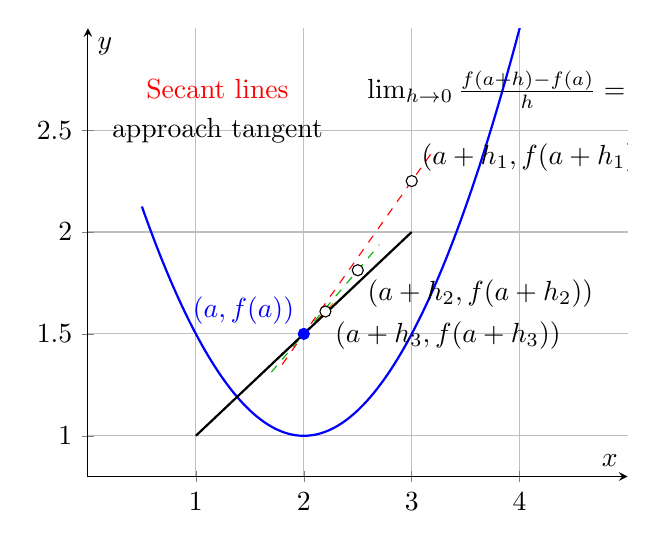
\begin{tikzpicture}

\pgfplotsset{
    soldot/.style={color=blue,only marks,mark=*},
    holdot/.style={color=black,fill=white,only marks,mark=*},
    compat=1.12
}
\begin{axis}[
    grid=both,
    axis lines=middle,
    ticklabel style={fill=white},
    xmin=0, xmax=5,
    ymin=0.8, ymax=3,
    xtick={1, 2, 3, 4},
    ytick={1, 1.5, 2, 2.5},
    xlabel=\(x\), ylabel=\(y\),
    samples=200
]
    % Main function curve
    \addplot[domain=0.5:4.5, blue, thick, smooth] {0.5*(x-2)^2 + 1};

    % Point of interest (a, f(a))
    \addplot[soldot] coordinates{(2,1.5)} node[above left] {$(a, f(a))$};

    % First secant line (h = 1)
    \addplot[domain=1.8:3.2, red, dashed] {0.75*(x - 2) + 1.5};
    \addplot[holdot] coordinates{(3,2.25)} node[above right] {$(a+h_1, f(a+h_1))$};

    % Second secant line (h = 0.5)
    \addplot[domain=1.7:2.7, green!70!black, dashed] {0.625*(x - 2) + 1.5};
    \addplot[holdot] coordinates{(2.5,1.8125)} node[below right] {$(a+h_2, f(a+h_2))$};

    % Third secant line (h = 0.2)
    \addplot[domain=1.9:2.3, orange, dashed] {0.55*(x - 2) + 1.5};
    \addplot[holdot] coordinates{(2.2,1.61)} node[below right] {$(a+h_3, f(a+h_3))$};

    % Tangent line
    \addplot[domain=1:3, black, thick] {0.5*(x - 2) + 1.5};

    % Labels
    \node at (axis cs:4.1,2.7) {\(\lim_{h \to 0} \frac{f(a+h)-f(a)}{h} = f'(a)\)};
    \node[red] at (axis cs:1.2,2.7) {Secant lines};
    \node at (axis cs:1.2,2.5) {approach tangent};
\end{axis}
  \end{tikzpicture}
  \end{document}
